\documentclass[11pt,a4paper]{article}
\usepackage[utf8]{inputenc}
\usepackage[T1]{fontenc}
\usepackage{lmodern}
\usepackage[margin=2.2cm]{geometry}
\usepackage{amsmath,amssymb,booktabs,tabularx,array,graphicx,xcolor,enumitem,hyperref}

% ---- fill these in before compiling ---------------------------------------------------------
\newcommand{\commithash}{\textcolor{red}{FILL IN: hash of the commit tagged final}}
\newcommand{\todo}[1]{\textcolor{red}{#1}}
% ---------------------------------------------------------------------------------------------
\newcommand{\zref}{z_{\mathrm{ref}}}
\newcommand{\zLP}{z_{\mathrm{LP}}}
\newcommand{\fone}{f_{\mathrm{CP1}}}
\setlength{\parindent}{0pt}\setlength{\parskip}{4pt}
\begin{document}\sloppy

\begin{center}
{\LARGE\bfseries Final report}\\[4pt]
{\large Introduction to Optimization}
\end{center}

\begin{tabularx}{\textwidth}{@{}lX@{}}
\toprule
Team & T10 \\
Storyline, variant & B (cloud resource allocation), variant 2; instance \texttt{cp34\_instance(10, 'B', 2)} \\
Members & Abdimazhit Inkar, Hafizi Nazifullah, Shaken Daniyal, Telgarin Diar \\
Repository & \url{https://github.com/1nkarych/Checkpoint2} \\
Tag and commit hash & \texttt{final}, \commithash \\
\bottomrule
\end{tabularx}

Notation: $S$ servers, $M$ virtual machines (VMs); own instance $S=11$, $M=50$; $\zLP=8.339506$, $\zref=8.382826$ (\texttt{results/ref\_values.json}, reproduced by \texttt{results/final\_exact.csv}). CP$n$ = Checkpoint $n$. The file behind every table is named under it.

\section{From the Checkpoint~1 model to the reference model}

\subsection*{Table 1. Element by element}
{\small
\begin{tabularx}{\textwidth}{@{}p{2.5cm}Xp{1.4cm}X@{}}
\toprule
Element & In Checkpoint~1 / in the reference model & Status & What it does to the meaning of the answer\\
\midrule
Assignment variables & $x_{ij}\in\{0,1\}$, VM $i$ on server $j$ / the same variable ($x_{ik}$, server $i$, VM $k$) & kept & Nothing: an answer is still one server for every VM.\\
Utilisation variables & $U_j=\max(U^{cpu}_j,U^{mem}_j)$ / one latency variable $t_i\ge 0$ per server, driven by CPU utilisation only & changed & Memory load no longer influences the cost; it only limits what is feasible.\\
Objective & $\min\sum_j (U_j+U_j^2)$ / $\min\sum_i t_i$, $t_i$ = maximum of four tangents of $u/(1-u)$ at $u=0,\,0.4,\,0.7,\,0.9$ & changed & The cost is linear in pieces: below $u=0.25$ every server has slope 1, so balancing there is free, while a server near $u=0.9$ costs 100 per unit of utilisation (ours: at most 3).\\
(1) One server per VM & $\sum_j x_{ij}=1$ / B1, 50 rows & kept & None.\\
(2) CPU capacity & $\sum_i r^{cpu}_i x_{ij}\le c^{cpu}_j$ / B2, 11 rows & kept & None.\\
(3) Memory capacity & $\sum_i r^{mem}_i x_{ij}\le c^{mem}_j$ / B3, 11 rows & kept & None as a constraint; it is now the only place where memory appears.\\
(4) Premium zone & $x_{ij}=0$ for a wrong zone / the same, as upper bounds 0 on 51 pairs & kept & None (7 premium VMs).\\
(5) Integrality & $x\in\{0,1\}$ / the same; relaxed to $[0,1]$ only to get $\zLP$ & kept & None; the relaxation gives the bound that our model did not have.\\
Latency rows & absent / B4: $t_i\ge a_m u_i-b_m$, 44 rows & added & They make the convex latency linear, so the model is a MILP that HiGHS solves with a proof.\\
Assumption 1: quadratic latency & $L(U)=U+U^2$ as an M/M/1-like approximation / piecewise-linear $u/(1-u)$ & changed & Our curve is too flat near full servers; the reference punishes them much harder.\\
Assumption 2: peak resource & latency follows the larger of CPU and memory utilisation / CPU only & dropped & A server with full memory and idle CPU is ``slow'' in our model and ``fast'' in the reference one.\\
Assumption 3: static, central & all 50 VMs placed at once / the same & kept & None.\\
Problem class & nonlinear binary program / mixed-integer linear program & changed & An exact optimum and a lower bound become available (CP3, Table 1).\\
\bottomrule
\end{tabularx}}

\subsection*{Own objective on the reference solutions}
Our Checkpoint~1 objective $\fone=\sum_j(U_j+U_j^2)$ contains no part that the reference model lacks (it needs only the loads), so it was evaluated directly on both solutions; nothing had to be replaced.

\begin{tabularx}{\textwidth}{@{}X>{\raggedleft\arraybackslash}p{3.2cm}>{\raggedleft\arraybackslash}p{3.4cm}@{}}
\toprule
Solution & Value under the reference objective & Value under my Checkpoint~1 objective\\
\midrule
Optimum of the reference model ($\zref$) & 8.382826 & 9.987753\\
Best solution of the approximate methods (GA, seed 4) & 8.382826 & 10.688779\\
\midrule
\emph{Extra:} descent under $\fone$ started from the reference optimum & 13.719587 & 7.469753\\
\emph{Extra:} descent under $\fone$ started from the GA solution & 12.181729 & 7.459695\\
\bottomrule
\end{tabularx}
{\small\raggedright Source: \texttt{results/final\_block1.csv} (\texttt{final/src/block1.py}). The descent is a steepest descent over feasible transfers and swaps; it gives a local optimum of our model, not its proven optimum.}

\textbf{Order.} Under the reference objective the two solutions are tied (both equal $\zref$ to nine decimals), although they are different placements: 45 of the 50 VMs sit on another server. Under our objective the tie is broken: the HiGHS optimum is better by $0.701$ ($6.6\,\%$). So the order is not reversed, but an indifference of the reference model becomes a clear preference in ours. Over the ten GA runs $\fone$ lies between 10.19 and 11.62 and does not follow the reference cost: seed 2 (reference cost 8.4044) has $\fone=10.19$, better than seed 4 (reference cost $\zref$, $\fone=10.69$).

\subsection*{Conclusion}
Yes, with its own model the team would have chosen another solution. Between the two solutions of the table it would have preferred the HiGHS optimum (9.988 against 10.689), where the reference model sees no difference. More important, neither is good for our model: a simple descent under $\fone$ reaches 7.46, that is $25\,\%$ below the reference optimum's 9.988, and this placement costs 12.18 under the reference objective, $45\,\%$ above $\zref$. The reason is the dropped Assumption~2: memory is the fuller resource here (871/1725 = 50.5\,\% against 233/504 = 46.2\,\% for CPU), in the reference optimum the memory utilisation exceeds the CPU utilisation on 7 of 11 servers, so $\fone$ mostly balances memory, which the reference objective does not see, and it leaves the CPU loads uneven, which the reference objective punishes. The two models therefore answer different questions, and the difference matters for the answer.

\section{Comparison of the methods of the team}

\subsection*{Table 2}
{\small
\begin{tabularx}{\textwidth}{@{}Xrrrrrrrr@{}}
\toprule
Method & best & mean & worst & std & feas. & time, s & gap$_{\mathrm{ref}}$, \% & gap$_{\mathrm{LP}}$, \%\\
\midrule
\csname @@input\endcsname final_table2.tex
\bottomrule
\end{tabularx}}
\[
\mathrm{gap}_{\mathrm{ref}}=100\cdot\frac{z-\zref}{\zref},\qquad
\mathrm{gap}_{\mathrm{LP}}=100\cdot\frac{z-\zLP}{z}\qquad(\text{both for the mean cost } z).
\]
{\small\raggedright Sources: \texttt{results/final\_table2.csv}, built from \texttt{Telgarin\_runs.csv} (GA), \texttt{Hafizi\_runs.csv} (SA, final runs), \texttt{Shaken\_tuning.csv} (rows \texttt{compare-rule} and \texttt{random}), \texttt{Telgarin\_random.csv}, \texttt{final\_exact.csv}. Seeds 0--9, budget 100\,000; std with divisor $n-1$. The team has two methods: GA with repair (Telgarin, Abdimazhit) and SA with transfer moves (Hafizi, Shaken). Times are those of the Checkpoint~4 files, measured on different laptops; on one machine the reruns took 11.8~s (GA), 2.2~s (SA) and 30.8~s (random search) per run (\texttt{results/final\_solutions\_*.json}).}

\subsection*{Figure F1}
\begin{center}
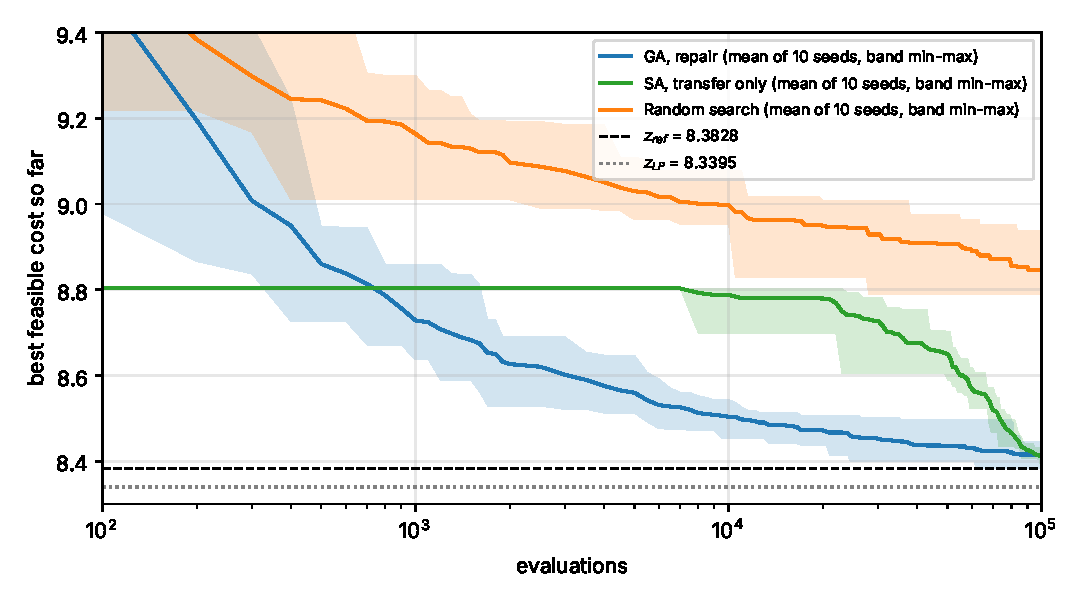
\includegraphics[width=0.8\textwidth]{final_F1.pdf}
\end{center}
{\small Best feasible cost so far, mean of seeds 0--9 with the min--max band (\texttt{results/final\_trace\_*.csv}: reruns of the Checkpoint~4 final runs, same seed gives the same final cost as in the Checkpoint~4 files). SA is the tuned configuration of the final runs.}

\subsection*{Analysis}
\textbf{The two methods do not differ in the mean.} GA: mean 8.4143, SA: 8.4117. The difference 0.0026 is 0.4 of its standard error (0.0065, from the stds 0.0184 and 0.0089 over 10 seeds) and seven times smaller than the GA std. Seed by seed SA is better on 4 seeds and GA on 6. What differs is the spread: the SA range $[8.3919,\,8.4258]$ lies inside the GA range $[8.3828,\,8.4459]$. GA is the only one of the two final configurations that reached $\zref$ (seed 4), and it also has the worst run. Both are far better than random search: the worst run of each (8.4459, 8.4258) is below the best random run (8.7888).

\textbf{Mechanism 1, the neighbourhood (common limit).} The worst-seed checks of two different members give the same picture. GA, seed 8, cost 8.4459 (Telgarin and Abdimazhit, CP4 Table~2 and question~4): 0 improving transfers, 20 improving swaps; the best swap gains 0.0309 and three steepest moves reach $\zref$. SA, seed 6, cost 8.4258 (Hafizi, CP4 Table~2; Shaken, question~4): 0 improving transfers, 8 improving swaps. Both methods stop in a local optimum of the transfer neighbourhood that is not a local optimum of the swap neighbourhood. SA proposes only transfers; the GA mutation moves one or two VMs and can make a given swap only by chance. This, and not the algorithm around it, explains why both end 0.3--0.4\,\% above $\zref$.

\textbf{Mechanism 2, budget and schedule (the shape of F1).} GA is within 1\,\% of its final mean after 11\,\% of the budget and gains only 0.0015 in the last 10\,\% (CP4 Telgarin, question~3): it is stuck, not short of budget. SA follows its cooling: 8.650 at 50\,000 evaluations, 8.426 at 90\,000, 8.412 at the end, still improving in the last 5\,\% (CP4 Hafizi, question~3). At any budget below about 90\,000 evaluations GA is therefore the better method; at the full budget they meet.

\textbf{Mechanism 3, tuning.} The SA row of the final runs is not the best SA we have. The Nelder--Mead tuning on seeds 100--104 chose $T_0=1.057$, $T_{end}=0.0105$; on seeds 0--9 the rule-based pair ($T_0=2.109$, $T_{end}=0.0037$) is better on 9 of 10 seeds (mean 8.3975 against 8.4117; CP4 Shaken, tuning table). Against GA the rule-based SA is better by 0.0168, about 2.6 standard errors, and reaches $\zref$ on seed 6. So the ranking ``SA $\approx$ GA'' holds for the tuned parameters only; with the rule-based temperatures SA is ahead, and the tuning lost more (0.17 points of gap$_{\mathrm{ref}}$) than the choice between GA and SA matters (0.03 points).

\textbf{Mechanism 4, repair.} Repaired random candidates give 8.8468, unrepaired ones 9.2093 (only about 4\,\% of them are feasible, \texttt{Shaken\_tuning.csv}); inside the GA, repair gave 8.4213 against 8.4469--8.4866 with a penalty (CP4 Abdimazhit, Section~5, five seeds, ranges overlap: a tendency). Repair helps, but it is not what separates GA from SA: SA never leaves the feasible set at all.

\textbf{The bound.} The gap of the relaxation itself is 0.52\,\% (the exact row). Of the 0.86--0.89\,\% gap$_{\mathrm{LP}}$ of the methods, 0.52 points belong to the bound and only 0.34--0.38 to the methods.

\section{Scaling}

Sizes $M=100,\,200,\,400$ (\texttt{scaled\_instance('B', M, 2)}; $S=29,\,57,\,114$). Budget 100\,000 evaluations, seeds 0--9. Parameters are those of the Checkpoint~4 final runs, unchanged: GA with repair, $N=30$, $p_c=0.9$, 1--2 mutated components, tournament 2, elitism 1; SA with transfer moves, $T_0=1.0570$, $T_{end}=0.010474$. Exact method: our Checkpoint~3 model built by \texttt{build\_model(d)} for the scaled instance and solved by HiGHS through \texttt{scipy.optimize.milp} with the options of \texttt{exact\_helper.solve\_milp}, limit 120~s. \textbf{Rounding rule} for the start: solve the LP relaxation; take the VMs in the order of decreasing CPU requirement; put each VM on the allowed server with the largest LP value $x_{ik}$ that still has room in CPU and memory; if no server with $x_{ik}>0$ has room, on the allowed server with room and the lowest CPU utilisation. The result is feasible for all sizes and is passed through the argument \texttt{start}.

\subsection*{Table 3}
{\footnotesize\setlength{\tabcolsep}{4pt}
\begin{tabular}{@{}llrrrrrlr@{}}
\toprule
Size & Method & \multicolumn{2}{c}{Value} & Best & \multicolumn{2}{c}{Gap to best known, \%} & Solver gap, \% & Time,\\
 & & best & mean & known & of best & of mean & (exact only) & s\\
\midrule
\csname @@input\endcsname final_table3.tex
\bottomrule
\end{tabular}}

{\small\raggedright Sources: \texttt{results/final\_table3.csv}, built from \texttt{final\_exact.csv}, \texttt{final\_GA\_repair.csv}, \texttt{final\_SA\_scaling.csv}. Best known = best value over all our runs of that size. Gap to best known $=100\,(z-z_{best})/z_{best}$. Solver gap $=100\,(z-\text{best bound})/|z|$ of HiGHS; it is not gap$_{\mathrm{LP}}$. For orientation, $\zLP$ of the three sizes is 9.0421, 24.6764, 54.4773 and the best bound of HiGHS is 9.1767, 24.8654, 54.8453. All 120 approximate runs are feasible. Times of the GA rows with the own start come from another machine than the rest.}

\subsection*{Figure F2}
\begin{center}
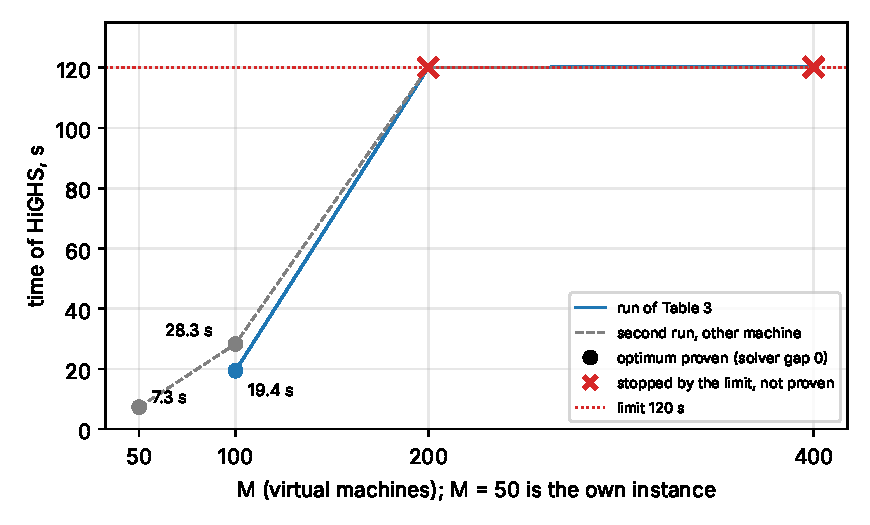
\includegraphics[width=0.6\textwidth]{final_F2.pdf}
\end{center}

\subsection*{Analysis}
\textbf{Where the exact solver stops proving.} At $M=50$ and $M=100$ HiGHS proves the optimum (solver gap 0) in 7~s and 28~s. At $M=200$ it runs into the limit with a solver gap of 0.12\,\%: the optimum is not proven, but the incumbent 24.8950 is the best value we know. At $M=400$ the limit leaves a gap of 11.6\,\%. So, between the sizes we tried, the proof is lost between 100 and 200.

\textbf{Where the approximate methods overtake the incumbent.} Not at 200: every one of the 40 approximate runs is worse than the incumbent (best 25.0240, 0.52\,\% above; means 0.9--1.3\,\% above). At 400 all 40 runs are better: the worst of them (55.9863) is 9.8\,\% below the incumbent 62.0512. Even the rounded LP solution without any search (60.7169, \texttt{results/final\_lp\_rounding.csv}) beats the incumbent. The crossover lies between 200 and 400. The exact solver remains useful at 400 through its bound: 54.8453 shows that our best known value 55.5651 is at most 1.3\,\% from the optimum.

\textbf{GA against SA.} At 400 they are equal: means 55.74 for both with stds near 0.1. At 200 GA is better by about 0.08 (25.152 against 25.229, stds 0.063 and 0.038, about 3 standard errors). At 100 the SA row needs care: with its own start no SA run improved the start at all (\texttt{results/final\_SA\_start\_check.csv}, 0 of 10 runs). The greedy construction that builds the start already costs 9.1767--9.1816 and is optimal on 5 of 10 seeds, so the 0.03\,\% is the result of the constructive heuristic, not of annealing. On the own instance and at 200 and 400 SA improves its start in all 10 runs.

\textbf{What the LP-rounded start changed.} For GA: nothing we can separate from the noise (100: 9.224 against 9.219; 200: 25.152 against 25.114, 1.7 standard errors; 400: 55.744 against 55.759). For SA at 200 and 400: nothing (25.229 against 25.203; 55.742 against 55.728). For SA at 100 it made the result worse, 9.2397 against 9.1791: the tuned $T_0$ accepts most worsening moves at the beginning (63.9\,\% in the first 5\,\% of the run on the own instance, CP4 Shaken, Table~2), so SA forgets any start, and from the rounded start it cannot come back to the quality of its own greedy start. The rounded solution is a poor start anyway (10.34, 27.08, 60.72: 9--13\,\% above the best known), and both methods erase it early.

\textbf{What three sizes cannot show.} We have one instance per size and one run of the solver each, so ``between 100 and 200'' and ``between 200 and 400'' are intervals, not thresholds, and nothing can be said beyond 400. The time limit hides the growth law: two of the four points in F2 are simply the limit, so no curve can be fitted. The scaled instances are also looser than our own (CPU fill 28--36\,\% against 46\,\%), so size and fill change together. An additional experiment would use sizes 125, 150, 175 and 250, 300, 350 with several instances per size, and the limit raised to 600~s at $M=200$ to see whether the 0.12\,\% closes; a second series at fixed $M$ with capacities scaled down would separate the effect of the fill ratio.

\section{Method-selection memo}

\textbf{To:} the owner of the VM placement problem. \textbf{From:} team T10. \textbf{Subject:} which solver to use for which size.

{\small
\begin{tabularx}{\textwidth}{@{}p{1.6cm}XXX@{}}
\toprule
 & Own instance & Medium scaled & Large scaled\\
\midrule
Problem & 50 VMs on 11 servers, 7 premium VMs tied to a zone; CPU fill 46\,\%, memory 50\,\% & 200 VMs on 57 servers; CPU fill 33\,\% & 400 VMs on 114 servers; CPU fill 36\,\% \\
Method & Exact solver (HiGHS on the linear model) & Exact solver stopped at 120~s; its incumbent is used & Simulated annealing (transfer moves), 10 seeds, best run taken; HiGHS run alongside only for the bound\\
Result and its level (gap) & 8.3828, proven optimal (solver gap 0) in 7~s. SA and GA: 0.34\,\% and 0.38\,\% above on average & 24.8950, at most 0.12\,\% above the optimum (solver gap; not proven). GA and SA: 0.5--1.3\,\% worse & 55.5809 best of 10 SA runs, mean 55.7424; best known 55.5651 (a GA run). At most 1.3--1.6\,\% above the optimum (bound 54.8453). Exact incumbent: 62.05, 11.7\,\% worse\\
Check & Checker \texttt{evaluate\_B} reports no violation; value equals the LP-based reference of Checkpoint~3; GA reaches the same value independently & Checker passes; the gap is read from the best bound of the solver, not from the word ``Optimal'' & Checker passes on 10 of 10 runs; fixed seeds reproduce the costs; spread between seeds 0.6\,\% (55.58--55.90) \\
Risk & None for the value. Solve time may vary between machines & 0.12\,\% may remain; a different instance of this size may end with a larger gap at the same limit & No proof; the result depends on the seed, so one run can be 0.6\,\% worse than the best; SA parameters were tuned on the small instance\\
\bottomrule
\end{tabularx}}

\subsection*{Recommendation for the real situation}
Use the exact solver with a time limit as the first tool and look at its solver gap. Up to about 100 VMs it returns the proven optimum in under half a minute, and at 200 VMs its unproven answer is still better than anything our heuristics found, so there is no reason to accept a heuristic there. When the gap after the limit is large (11.6\,\% at 400 VMs), switch to simulated annealing with 10 seeds and keep the solver's bound as the quality certificate. We prefer SA to the genetic algorithm for this role because at 400 VMs the two give the same quality (mean 55.74 for both), while SA is the simpler program, needs no repair procedure and ran faster (8~s against 13~s per run on the same machine). GA is not wrong, it is just not better; at 200 VMs it was slightly ahead of SA, but there the exact solver beats both. Random search is never an option (5.5\,\% above the optimum on the own instance). One caution for SA: use the rule-based temperatures, not the tuned ones; on the own instance the tuned pair was worse on 9 of 10 seeds.

\subsection*{What would change the recommendation}
\emph{Size and time.} The switch from the exact solver to SA is decided by one measurable number: the solver gap at the end of the time limit. Below about 1\,\% (the level SA and GA reach) keep the exact incumbent; above it take SA. In our data this happens between 200 and 400 VMs for a limit of 120~s; a longer limit moves the switch to larger sizes.
\emph{Fill ratio.} All our instances are loose (CPU fill 28--46\,\%, memory at most 50\,\%). If the fill ratio approaches 100\,\%, as in the heaviest instances of Checkpoint~3, the recommendation for large sizes is no longer supported: the SA start is built by a greedy rule that may fail to find any feasible placement, transfer moves are mostly blocked on full servers (a swap move would be needed, and both methods already lack it), and the GA repair returns an unrepaired individual when no VM can be moved. The measurable trigger is the number of feasible runs: if fewer than 10 of 10 runs are feasible, or the fill ratio exceeds about 90\,\%, we would first add the swap move and re-run the comparison, and until then rely on the exact solver with a longer limit, whose answer is at least feasible by construction.
\emph{Objective.} If the owner's latency really depends on memory as well as on CPU (our Checkpoint~1 assumption), the whole ranking has to be redone: Section~1 shows that the best placement for one objective is 45\,\% worse for the other.

\appendix
\section{Authorship}
\begin{tabularx}{\textwidth}{@{}XXXXl@{}}
\toprule
Block & Wrote the code & Ran the experiment & Wrote the text & Signature\\
\midrule
1. Model & \todo{name} & \todo{name} & \todo{name} & \todo{name}\\
2. Comparison & \todo{name} & \todo{name} & \todo{name} & \todo{name}\\
3. Scaling & \todo{name} & \todo{name} & \todo{name} & \todo{name}\\
4. Memo & \todo{name} & \todo{name} & \todo{name} & \todo{name}\\
\bottomrule
\end{tabularx}

\section{Declarations}
External code and the use of AI assistants are declared in \texttt{README.md} of the repository, section ``Final -- declarations'', one table per author:\\ \url{https://github.com/1nkarych/Checkpoint2\#final--declarations}

\end{document}
